\subsection{Problem}

\renewcommand{\theequation}{\theenumi}
\begin{enumerate}[label=\thesection.\arabic*.,ref=\thesection.\theenumi]
\numberwithin{equation}{enumi}
	\item If A and B are two independent events, then the probability of occurrence of at least one of A and B is given by 1- P(A')P(B').\\
	\solution If two events A and B are independent,\\
	\begin{align}
	P\brak{A\cap B} &= P\brak{A} . P\brak{B} \label{eq:ind}
	\end{align}
	$P\brak{\text{atleast one of A and B}} = P\brak{A\cup B}$	\\
	\begin{align}
	P\brak{A\cup B} &= P\brak{A} + P\brak{B} - P\brak{A\cap B}	\\
	P\brak{A\cup B} &= P\brak{A} + P\brak{B} - P\brak{A} . P\brak{B} \\
	P\brak{A\cup B} &= P\brak{A} + P\brak{B} \brak{1 - P\brak{A}}\\
	P\brak{A\cup B} &= P\brak{A} + P\brak{B} P\brak{A'}\\
	P\brak{A\cup B} &= 1 - P\brak{A'} + P\brak{B} P\brak{A'}\\
	P\brak{A\cup B} &= 1 - P\brak{A'} \brak{1 - P\brak{B}}\\
	\therefore P\brak{A\cup B} &= 1 - P\brak{A'} P\brak{B'}
	\end{align}
	
\begin{comment}	
The following python code computes the area of $\triangle$ABC in Fig.\ref{fig:qfour}.
	\begin{lstlisting}
	./codes/quadrilateral/q4.py
	\end{lstlisting}
	
	
	\begin{figure}[!ht]
	\centering
	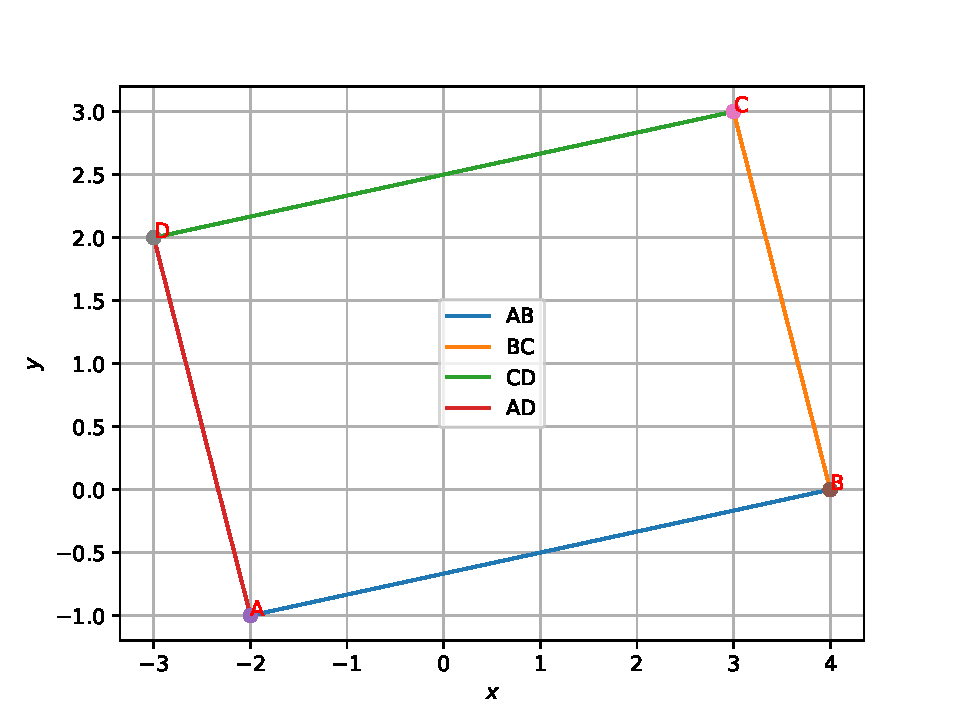
\includegraphics[width=\columnwidth]{./figs/quadrilateral/q4.pdf}
	\caption{Parallelogram of Q.2.2.5}
	\label{fig:qfour}	
	\end{figure}
	
\end{comment}	
\end{enumerate}
